\documentclass{article}
\usepackage[english,german]{babel}
\usepackage{graphicx}
\usepackage{amssymb}
\usepackage[utf8]{inputenc}
\usepackage{amsmath}

\begin{document}

\title{Hausarbeit SME-PHY-B: Wahlthema 2 - Fitnesszähler}
\author{Joel Ewig}
\date{\today}
\maketitle
\clearpage

\begin{abstract}
Sensorbasiert sollen ähnlich einer Fitnessuhr verschiedene SportÜbungen erkennt sowie die Anzahl wie oft diese jeweils ausgeführt wurden.
Benutzt werden sollen der Beschleunigungssensor und das Gyroskop des IMU-6050.\\
Mein Lösungsansatz gliedert sich in mehrere Stufen:
die Rohdaten aus dem IMU-6050 sollten durch einen mehrdimensionalen Kalman-Filter bereinigt werden.
Die bereinigten Daten werden mit dem K-Means Algorithmus geclustert um daraus sogenannte \glqq{}Beobachtungen\grqq{} zu machen.
In der Lernphase wird mit diesen Beobachtungen pro Übung ein Hidden Markov Model erlernt.
In der folgenden Detektionsphase werden die empfangenen Daten ebenfalls geclustert und die Beobachtungen an alle Hidden Markov Modelle weitergegeben.
Das HMM welches die höchste Wahrscheinlichkeit für die Emittierung der beobachteten Folge bestimmt, gilt als Erkenner und die zugehörige Übung wird als ausgeführt behandelt.
\end{abstract}
\clearpage

\tableofcontents
\clearpage

\section{Konzept}
\begin{enumerate}
\item Accelerometer und Gyrometer mittels mehrdimensionalenm Kalman-Filter bereinigt
\item gefilterte Daten werden mittels K-Means geclustert
\item clusterzugehörigkeit als beobachtung in ein HMM zur Erkennung von Aktivität und Zählen
\end{enumerate}
Es folgt ein Beispiel für eine typische Ausführung während der Detektionsphase:\\
Während der Ausführung einer Übung werden die Daten des Gyroskops und des Beschleunigungssensors erfasst.
Für 5 Zeitschritte haben die Gyroskopdaten die Form:
\begin{align*}
\left[\begin{array}{rrrrr}
g_{1}^1 & g_{1}^2 & g_{1}^3 & g_{1}^4 & g_{1}^5 \\
g_{2}^1 & g_{2}^2 & g_{2}^3 & g_{2}^4 & g_{2}^5 \\
g_{3}^1 & g_{3}^2 & g_{3}^3 & g_{3}^4 & g_{3}^5 \\
\end{array}\right]
\end{align*}
und die des Beschleunigungssensors die Form:
\begin{align*}
\left[\begin{array}{rrrrr}
a_{1}^1 & a_{1}^2 & a_{1}^3 & a_{1}^4 & a_{1}^5 \\
a_{2}^1 & a_{2}^2 & a_{2}^3 & a_{2}^4 & a_{2}^5 \\
a_{3}^1 & a_{3}^2 & a_{3}^3 & a_{3}^4 & a_{3}^5 \\
\end{array}\right]
\end{align*}
Diese werden mit einem mehrdimensionalen Kalman-Filter bereinigt und zusammengeführt, das sieht dann so aus:
\begin{align*}
\left[\begin{array}{rrrrr}
a_{1}^1 & a_{1}^2 & a_{1}^3 & a_{1}^4 & a_{1}^5 \\
a_{2}^1 & a_{2}^2 & a_{2}^3 & a_{2}^4 & a_{2}^5 \\
a_{3}^1 & a_{3}^2 & a_{3}^3 & a_{3}^4 & a_{3}^5 \\
g_{1}^1 & g_{1}^2 & g_{1}^3 & g_{1}^4 & g_{1}^5 \\
g_{2}^1 & g_{2}^2 & g_{2}^3 & g_{2}^4 & g_{2}^5 \\
g_{3}^1 & g_{3}^2 & g_{3}^3 & g_{3}^4 & g_{3}^5 \\
\end{array}\right]
\end{align*}
Die Spaltenvektoren dienen als Eingabe für den K-Means Clustering Algorithmus.
Dieser gibt für jeden Spaltenvektor das zugehörige Cluster $c$ aus:
\begin{align*}
\left[\begin{array}{r}
a_{11}\\
a_{21}\\
a_{31}\\
g_{11}\\
g_{21}\\
g_{31}\\
\end{array}\right]
\rightarrow c_1
\end{align*}
Die Sequenz der Clusternamen dient als Eingabe in $n$ Hidden Markov Modelle, n ist dabei die Anzahl der Übungen, die erkannt werden sollen.
Die Hidden Markov Modelle geben eine Emissionswahrscheinlichkeit für die beobachtete Folge an:
\begin{align*}
\left[c_1, c_2, c_3, c_4, c_5\right] \rightarrow p_1, p_2, .. p_n
\end{align*}
Aus den Emissionswahrscheinlichkeiten $p$ wird die größte gewählt.
Die zum gewählten Hidden Markov Model gehörende Übung gilt als erkannt.

\section{Sensorik}
Auf dem Arduino werden die Daten des Beschleunigungssensors und des Gyroskop aus dem IMU ausgelesen.
Das Gyroskop sowie der Beschleunigungssensor werden dem im Datenblatt beschriebenem Selbsttest unterzogen.
Dieser soll feststellen, dass die Sensoren noch funktionsfähig sind.
Die zugehörigen Daten werden über die serielle Schnittstelle an ein Pythonskript übermittelt, welches die zugehörigen Rechnungen vornimmt und bei Nichtbestehen des Selbsttests das Programm beendet.

\section{Mehrdimensionaler Kalman-Filter}
Der mehrdimensionale Kalman-Filter soll hier vernachlässigt werden, da er nicht unbedingt nötig ist für die Erkennung.
Mit einem solchen Kalman-Filter wäre die Erkennung vermutlich robuster, da mit bereinigten Daten \glqq engere \grqq{} Cluster zu erwarten wären.
Hier wird aus Zeitgründen auf einen Kalman-Filter verzichtet, da dieser die Ergebnisse zwar verbessern würde, allerdings nicht unbedingt notwendig ist.\\
Ein solcher Filter würde wie folgt funktionieren;
\begin{align*}
X^{[t+1]} &= A^{[t]}X^{[t]} + B^{[t]}u^{[t]} + C^{[t]} + \epsilon^{[t]}\\
\left[\begin{array}{r}
a_{1}\\
a_{2}\\
a_{3}\\
g_{1}\\
g_{2}\\
g_{3}\\
\end{array}\right]^{[t+1]}
&= A^{[t]} \left[\begin{array}{r}
a_{1}\\
a_{2}\\
a_{3}\\
g_{1}\\
g_{2}\\
g_{3}\\
\end{array}\right]^{[t]}
+ B^{[t]}\left[\begin{array}{r}
ra_{1}\\
ra_{2}\\
ra_{3}\\
rg_{1}\\
rg_{2}\\
rg_{3}\\
\end{array}\right]^{[t]}
+ C^{[t]} + \epsilon^{[t]}
\end{align*}
Dabei müssen $A^{[t]}$, $B^{[t]}$ und $C^{[t]}$ gesetzt und experimentell überprüft werden.
$\epsilon^{[t]}$ modelliert das Messrauschen und ist damit bei der Implementierung nicht zu beachten, es darf allerdings nicht vergessen werden, dass der Kalman-Filter nur ein Zustands\textbf{schätzer} ist.

\section{Phasen}
Der Ansatz nutzt in der Praxis zwei Phasen.
In der Ersten, der Lernphase, wird die Anzahl der zu erkennenden Übungen sowie für jede Übung eine Anzahl an Ausführungen festgelegt.
Nachdem diese ausgeführt wurden und fertig verarbeitet wurden ist die Lernphase beendet.
In der Detektionsphase wird eine Anzahl an zu erkennenden Ausführungen festgelegt.
Nachdem diese ausgeführt wurden, wird das Ergebnis der Detektion ausgegeben und die Detektionsphase ist beendet.

\subsection{Lernphase}
Die einkommenden 6-dimensionalen Daten werden wie oben beschrieben mit einem K-Means geclustert.
Der K-Means wird auf den kompletten Trainingsdaten, also unabhängig von den Übungen, initialisiert.
Jeder Punkt bekommt dadurch einen Clusternamen zugewiesen, umgesetzt als Nummern, welche weitergegeben werden.
Die Clusternamen sind die Beobachtungen die als Eingabe für das Lernen der HMMs dienen.\\
Genutzt wird ein Hidden Markov Model $(\pi, p, q)$ mit:
\begin{enumerate}
\item $\pi: Z \rightarrow [0,1]$ als inititale Wahrscheinlichkeiten für die Zustände $Z$
\item $p: Z \times Z \rightarrow [0,1]$ als Übergangswahrscheinlichkeiten zwischen den Zuständen $Z$
\item $q: Z \times B \rightarrow [0,1]$ als Beobachtungswahrscheinlichkeiten für die Beobachtung $B$ in den Zuständen $Z$
\end{enumerate}
Ein HMM für eine Übung wird wie folgt trainiert:
Zuerst werden die Emissionswahrscheinlichkeiten und die Übergänge zwischen den versteckten Zuständen zufällig initialisiert, konkret wird also $\pi$ mit Zufallszahlen im Intervall $[0,1]$ gefüllt.
Anschließend werden die genannten Werte mittels des Baum-Welch Algorithmus an die in der Lernphase aufgenommenen Sequenzen angepasst, mehr dazu in Kapitel \ref{sec:BaumWelch}.
Die HMMs werden mehrfach initialisiert um zu die Wahrscheinlichkeit zu vermindern, dass man nicht über ein lokales Optimum hinauskommt.
Es wird das HMM gewählt, welche die größte Wahrscheinlichkeit bei der Erkennung der bekannten Übungen aufweist.
Durch die geringe Anzahl an Lerndaten, wird hier keine Mindestwahrscheinlichkeit gesetzt, da dazu zu wenig Trainingsdaten vorhanden sind.
In den durchgeführten Experimenten hat sich kein Wert als stabil erwiesen.
Das liegt an dem Ziel, mit möglichst wenigen Übungen in der Lernphase auszukommen, dadurch bleibt der Trainingsdatenumfang relativ gering.

\subsection{Detektionsphase}
In der Detektionsphase werden die empfangenen Daten mit dem K-Means aus der Lernphase geclustert.
Der K-Means ist eingefroren, das heißt die Clustermittelpunkte bleiben wie sie in der Lernphase festgestellt wurden.\\
Die Beobachtungen einer Durchführung werden allen HMMs zugeführt, diese geben die Emissionswahrscheinlichkeit für die beobachtete Sequenz aus.
Es wird die Übung erkannt, dessen zugehöriges HMM die höchste Wahrscheinlichkeit für die Emission der beobachteten Sequenz ausgibt.

\section{Baum-Welch Algorithmus}
\label{sec:BaumWelch}
Der Baum-Welch Algorithmus wendet den Maximum-Likelihood Algorithmus auf Hidden Markov Modelle an.
Genutzt wird ein Hidden Markov Model $(\pi, p, q)$ mit:
\begin{enumerate}
\item $\pi: Z \rightarrow [0,1]$ als inititale Wahrscheinlichkeiten für die Zustände $Z$
\item $p: Z \times Z \rightarrow [0,1]$ als Übergangswahrscheinlichkeiten zwischen den Zuständen $Z$
\item $q: Z \times B \rightarrow [0,1]$ als Beobachtungswahrscheinlichkeiten für die Beobachtung $B$ in den Zuständen $Z$
\end{enumerate}
In der hier genutzten Implementierung sind $p$ und $q$ als Matrizen umgesetzt.
Diese werden zu Beginn mit zufälligen Werten initialisiert.
Im ersten Schritt werden die Wahrscheinlichkeiten mit den aktuellen Parametern ermittelt.
Die Idee hinter dem Baum-Welch Algorithmus ist, die Übergänge, die der wahrscheinlichste Pfad durch das HMM nutzt, wahrscheinlicher zu machen.\\
Für eine beobachtete Sequenz $O = {o_1, .., o_T}$ heißt das, dass $\pi_i$ in der nächsten Iteration zu $\tilde{\pi}$ und berechnet sich durch:
\[
\tilde{\pi_i} = \gamma_i(1)
\]
$\gamma_i(t)$ ist die erwartete Häufigkeit, sich in Zustand $i$ zum Zeitpunkt $t$ aufzuhalten.
Diese ergibt sich aus:
\[
\gamma_i(t) = \frac{\alpha_i(t)\beta_i(t)}{\sum_{j=1}^{N}\alpha_j(t)\beta_j(t)}
\]
$\alpha$ und $\beta$ können rekursiv ermittelt werden über:
\begin{align*}
\alpha_i(1) &= \pi_iq_i(o_1) \\
\alpha_j(t+1) &= \sum_{i=1}^{N}\alpha_i(t)p(i, j)q_j(o_{t+1})\\
\beta_i(T) &= 1 \\
\beta_i(t) &= \sum_{j=1}^{N}p(i, j)q_j(o_{t+1})\beta_j(t+1)
\end{align*}
Dann werden $p$ und $q$ angepasst mit:
\begin{align*}
p(i, j) &= \frac{\text{Anzahl der Übergänge von i nach j}}{\text{Anzahl der Übergänge von i zu einem beliebigen Zustand}}\\
\\
q_i(k) &= \frac{\text{Anzahl der Zeitschritte in i in denen k beobachtet wurde}}{\text{Anzahl der Zeitschritte in i}}
\end{align*}
Diese Operationen werden ausgeführt bis sich keiner der Werte um mehr als ein Mindestwert (hier: 0,01) verändert oder die festgelegte Höchstanzahl an Iterationen (hier: 100) erreicht ist.



\section{Evaluation}

Experimentell wurde ermittelt, dass stabile Ergebnisse für alle $k \geq 3$  für einfache und wenige Übungen liefert.
Ab $k \geq 5$ auch mit mehr beziehungsweise voneinander unterschiedlicheren Übungen, weshalb $k = 5$ als Default-Wert genutzt wird.
Für sehr komplexe Übungen sollte $k$ erhöht werden.\\
FÜ
\begin{figure}[htbp]
\centering
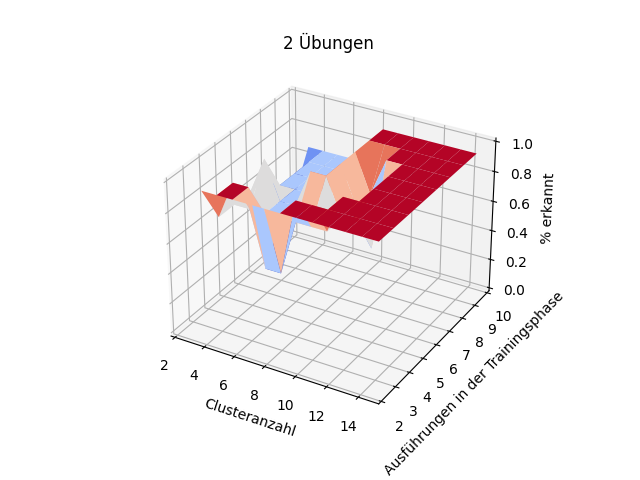
\includegraphics[width=0.7\textwidth]{figures/2_graph.png}
\end{figure}

\begin{figure}[htbp]
\centering
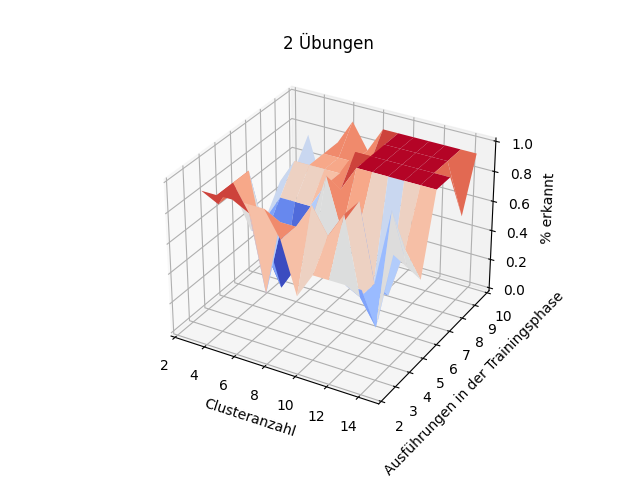
\includegraphics[width=0.7\textwidth]{figures/3_graph.png}
\end{figure}

\begin{figure}[htbp]
\centering
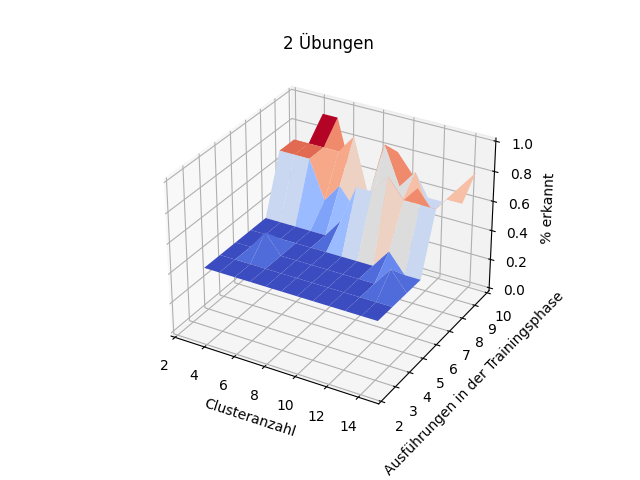
\includegraphics[width=0.7\textwidth]{figures/4_graph.png}
\end{figure}

\begin{figure}[htbp]
\centering
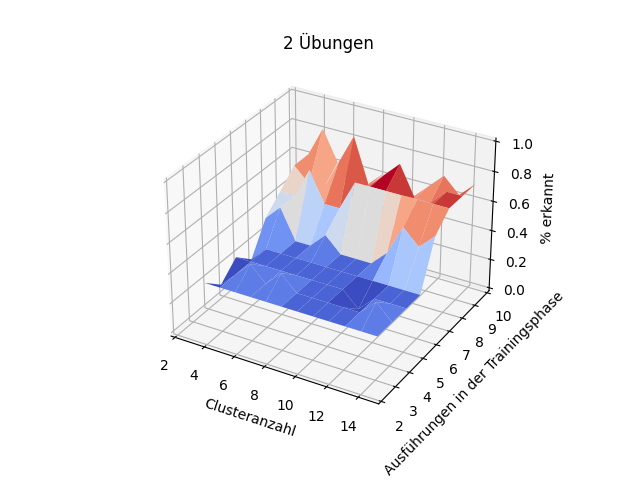
\includegraphics[width=0.7\textwidth]{figures/5_graph.png}
\end{figure}

\end{document}
